\documentclass[aspectratio=169]{beamer}

\usepackage{tikz}
\usetikzlibrary{arrows.meta}
\usetikzlibrary{shapes}

\beamertemplatenavigationsymbolsempty%

\definecolor{sblau}{HTML}{007ec1}
\definecolor{sgrau}{HTML}{e6e4e4}

\begin{document}

\begin{frame}
    \centering
    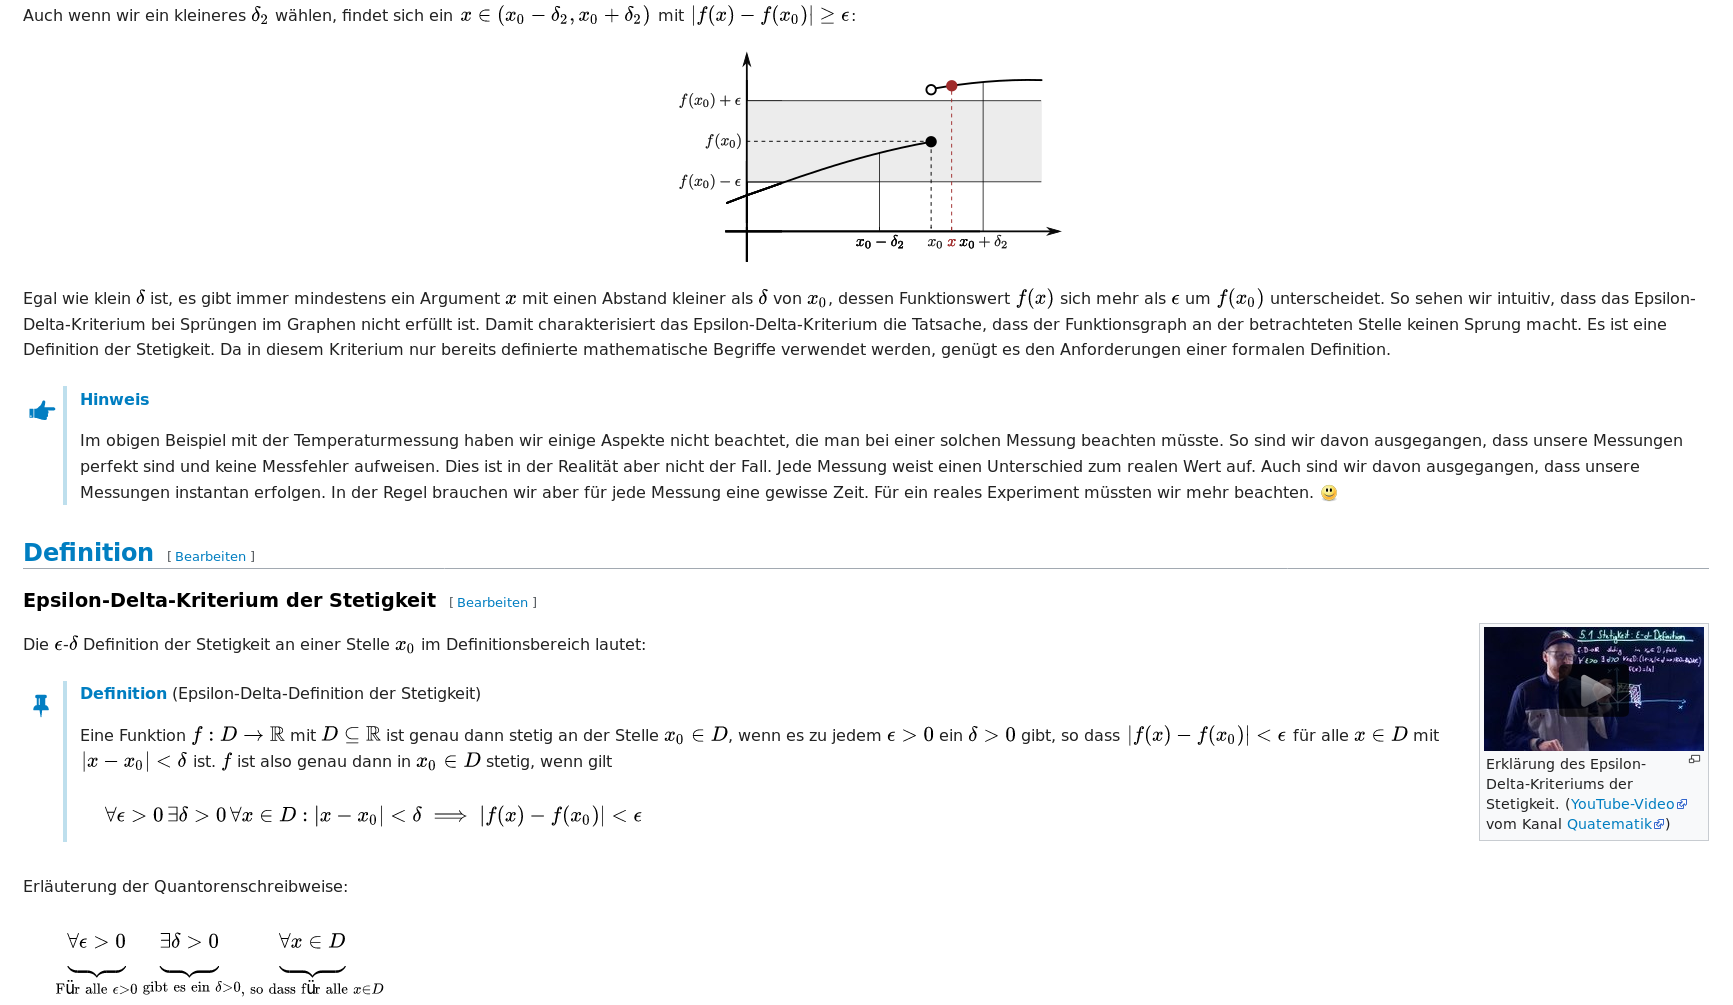
\includegraphics[height=0.9\textheight]{mfnf.png}
\end{frame}

\begingroup
%\setbeamercolor{background canvas}{bg=sgrau}
\begin{frame}
    \centering
    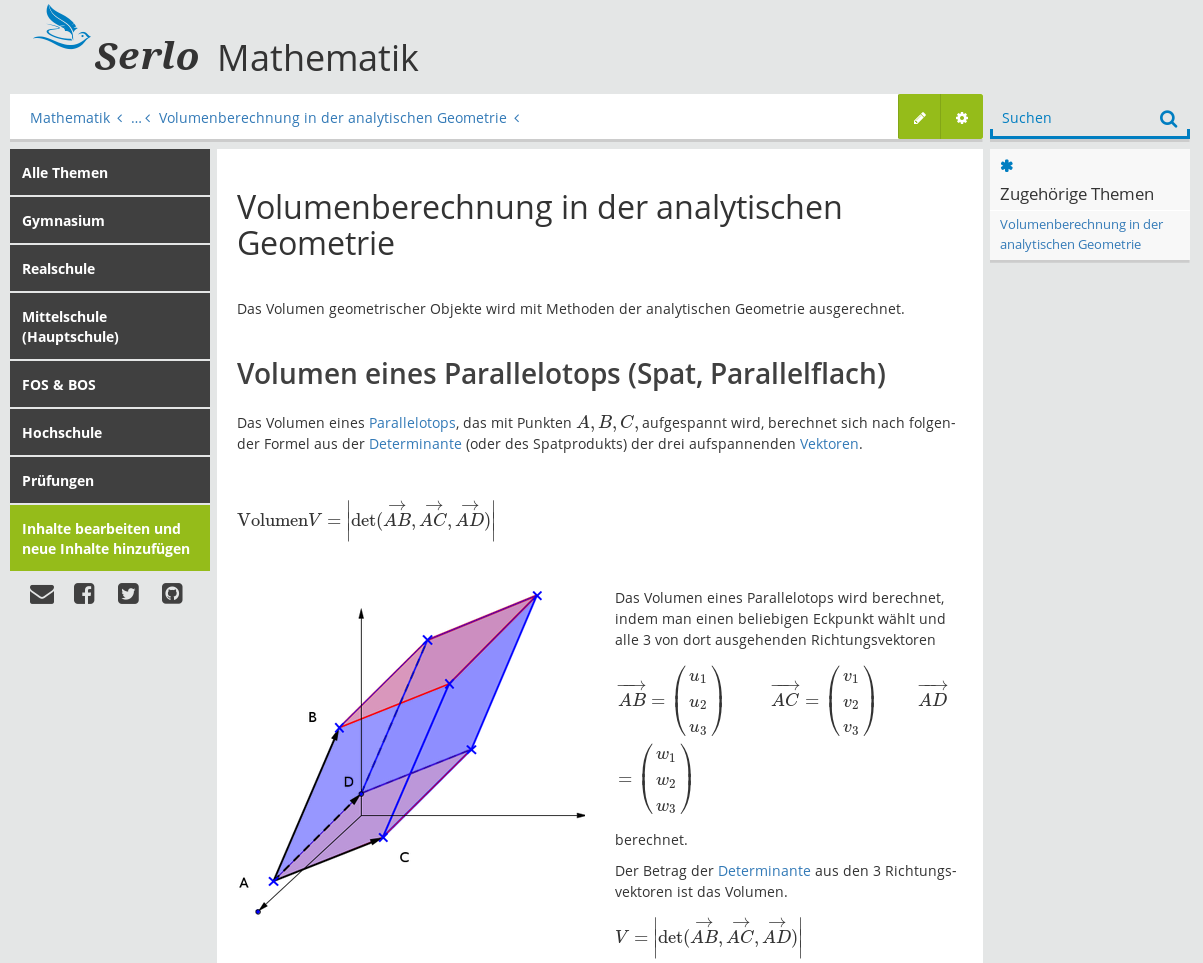
\includegraphics[height=0.9\textheight]{serlo.png}
\end{frame}
\endgroup

\begingroup
\setbeamercolor{background canvas}{bg=sblau}
\begin{frame}
    \centering
    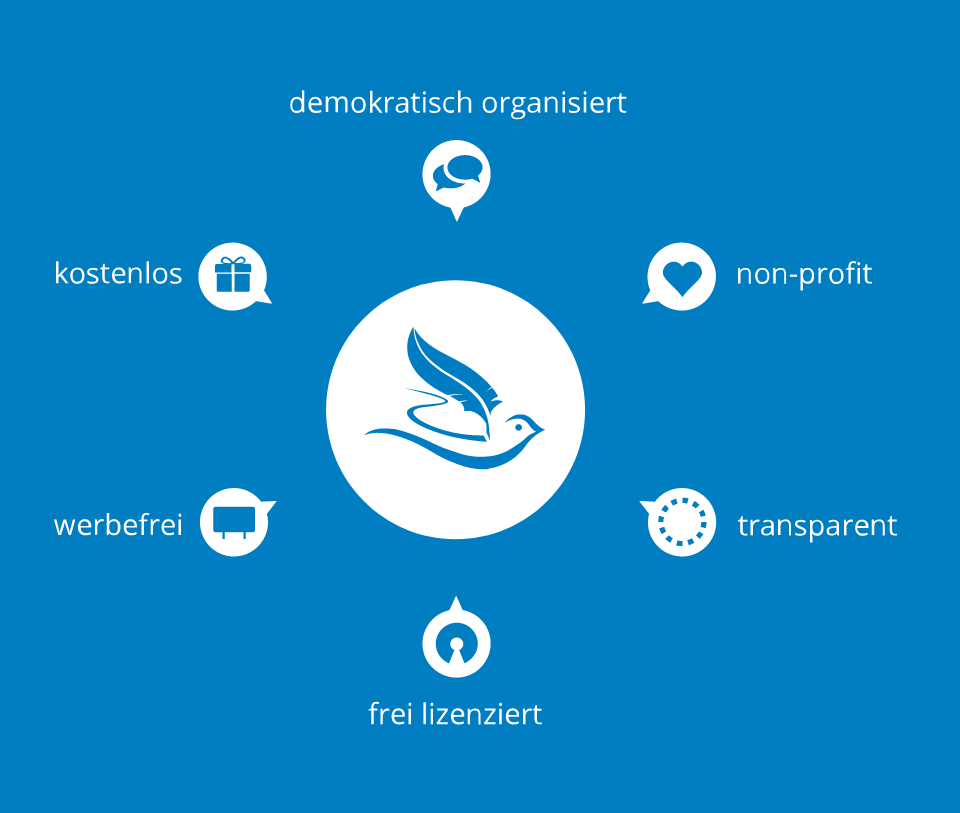
\includegraphics[height=\textheight]{serlo-vision.png}
\end{frame}
\endgroup

\begin{frame}
    \vfill

    \begin{minipage}[b]{0.3\textwidth}
        \centering
        
\includegraphics[width=3cm]{serlo-logo.png}
        \\[0.5em]
        783.934 Nutzer*innen\footnotemark[1]
    \end{minipage}
    \hfill
    \begin{minipage}[b]{0.3\textwidth}
        \centering
        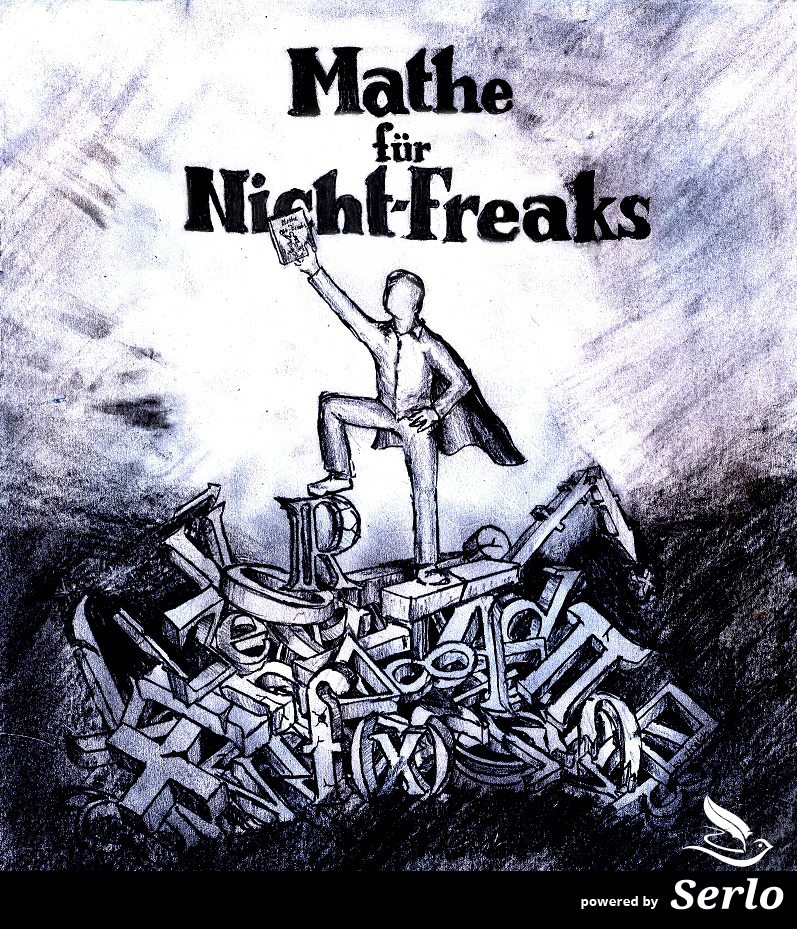
\includegraphics[width=3cm]{mfnf-logo.jpg}
        \\[0.5em]
        110.967 Nutzer*innen\footnotemark[1]
    \end{minipage}
    \hfill
    \begin{minipage}[b]{0.3\textwidth}
        \centering
        
\includegraphics[width=3cm]{serlo-abc-logo.png}
        \\[0.5em]
        500+ Installationen\footnotemark[1]
    \end{minipage}

    \begin{center}
        9300 Downloads \\ des PDF-Exports des Buchs Analysis 1
    \end{center}

    \footnotetext[1]{Pro Monat, Stand 2018}
\end{frame}

\begin{frame}
    \centering
    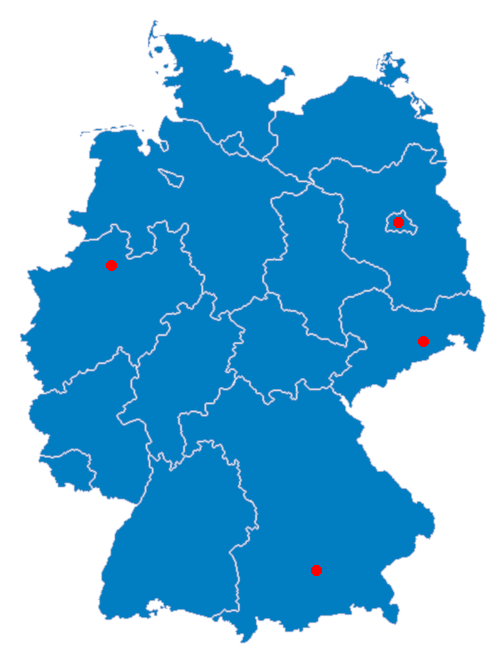
\includegraphics[height=0.8\textheight]{map.png}
    \begin{tikzpicture}[overlay]
        \node[anchor=east] (Berlin) at (3.8,4.65) {Berlin};
        \node[anchor=east] (Dresden) at (3.8,3.34) {Dresden};
        \node[anchor=east] (Munchen) at (3.8,0.83) {München};
        \node[align=left] (Munster) at (-9,4.18) {Münster};
        \draw[color=red] (Berlin.west) to (-1.26,4.65);
        \draw[color=red] (Dresden.west) to (-0.96,3.34);
        \draw[color=red] (Munchen.west) to (-2.2,0.83);
        \draw[color=red] (Munster.east) to (-4.4,4.18);
    \end{tikzpicture}
\end{frame}

\begin{frame}{}
    \centering
    \vfill
    
\includegraphics[width=.3\linewidth]{wikibooks.png}
    \hfill
    \LARGE
    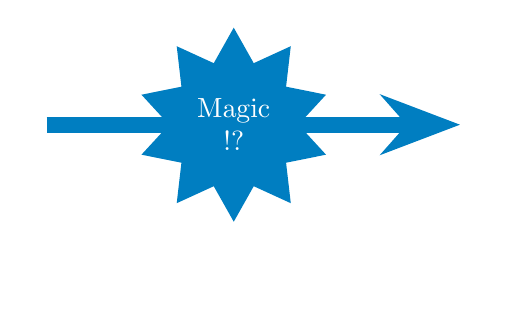
\begin{tikzpicture}[>={Stealth[sblau]}]
        \node[node distance=3cm] (E) at (3, 0) {};
        \node[node distance=3cm] (I) at (-2.5, 0) {};
        \path[->, line width=2mm, sblau](I) edge (E);
        \node[shape=star, ultra thick, white, fill=sblau, star points = 10, align=center] (M) {Magic\\!?};
        \node[] (DUMMY) at (0, -2) {};
    \end{tikzpicture}
    \hfill
    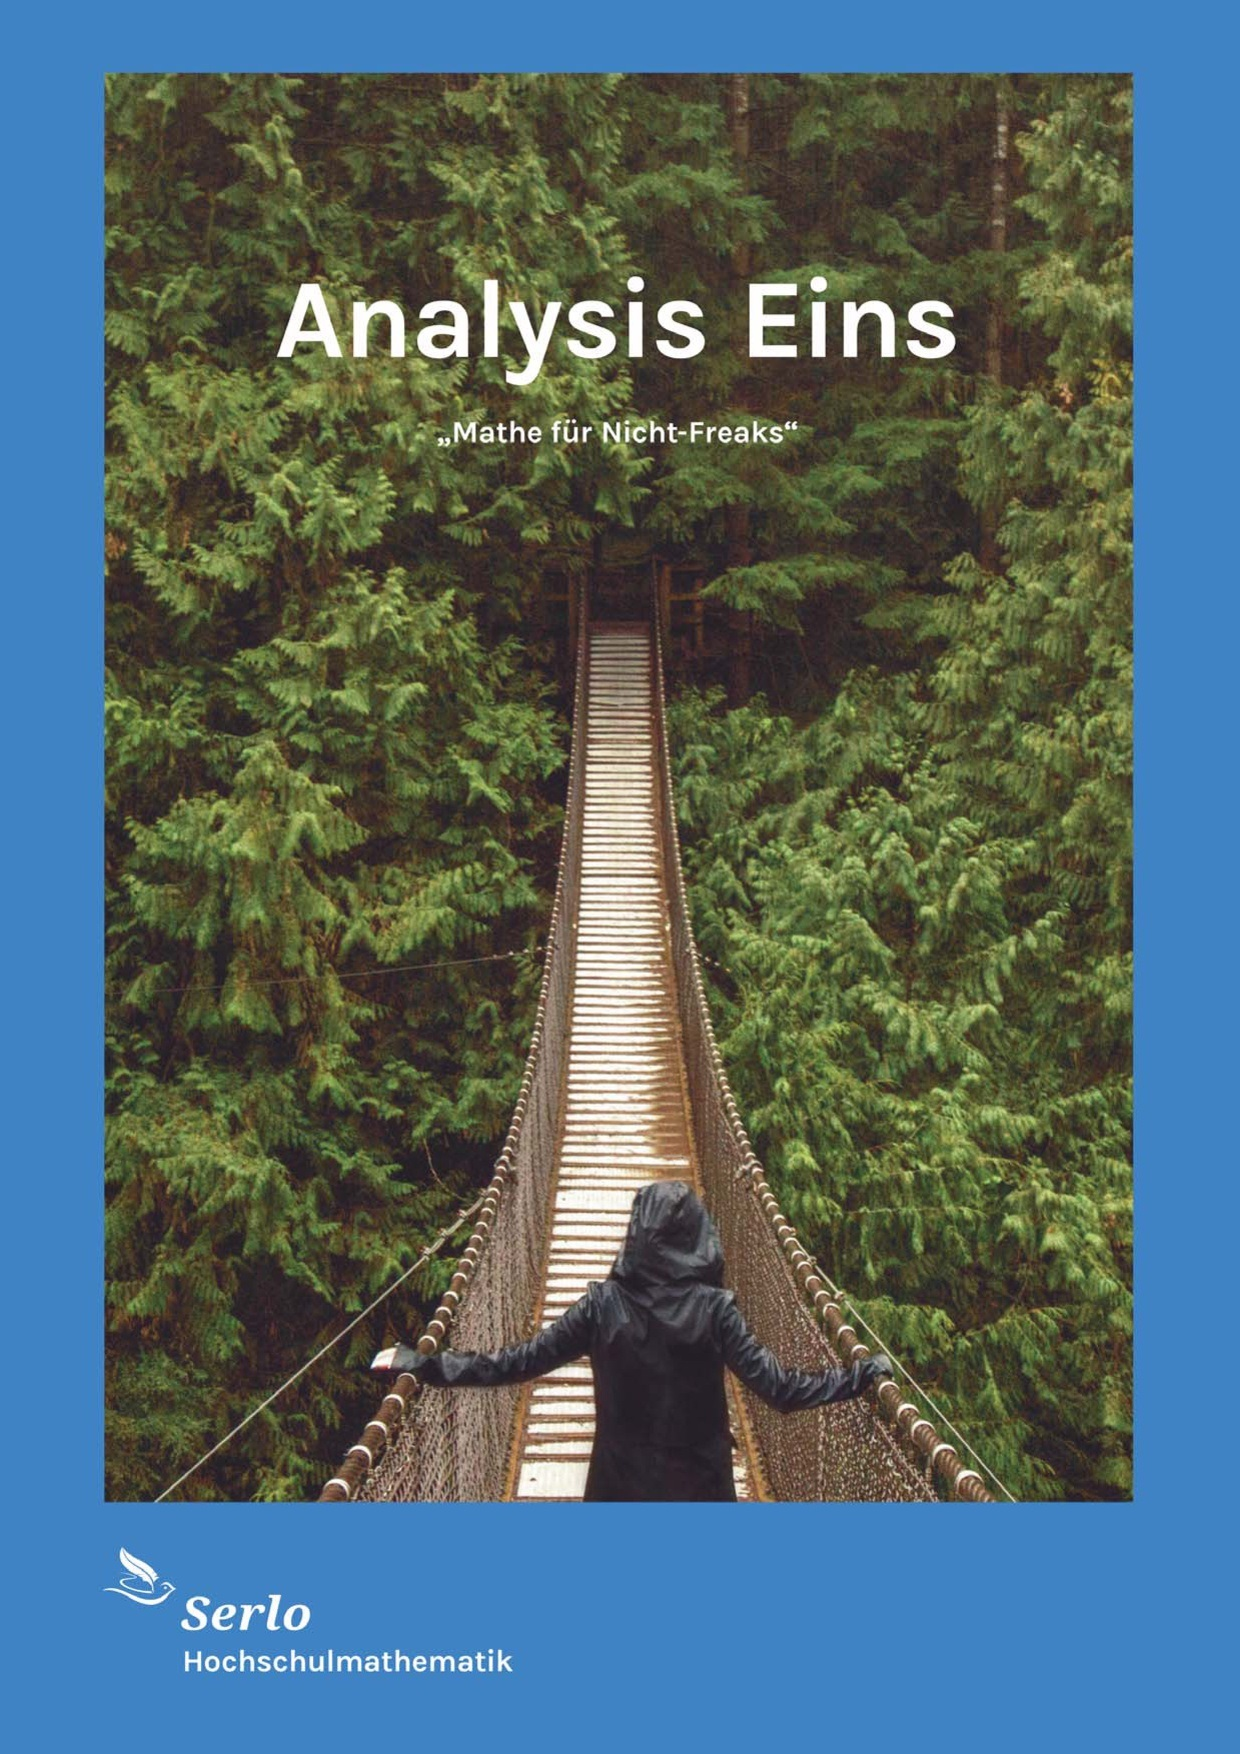
\includegraphics[width=.25\linewidth]{cover.jpg}
\end{frame}

\begin{frame}{}
    \centering
    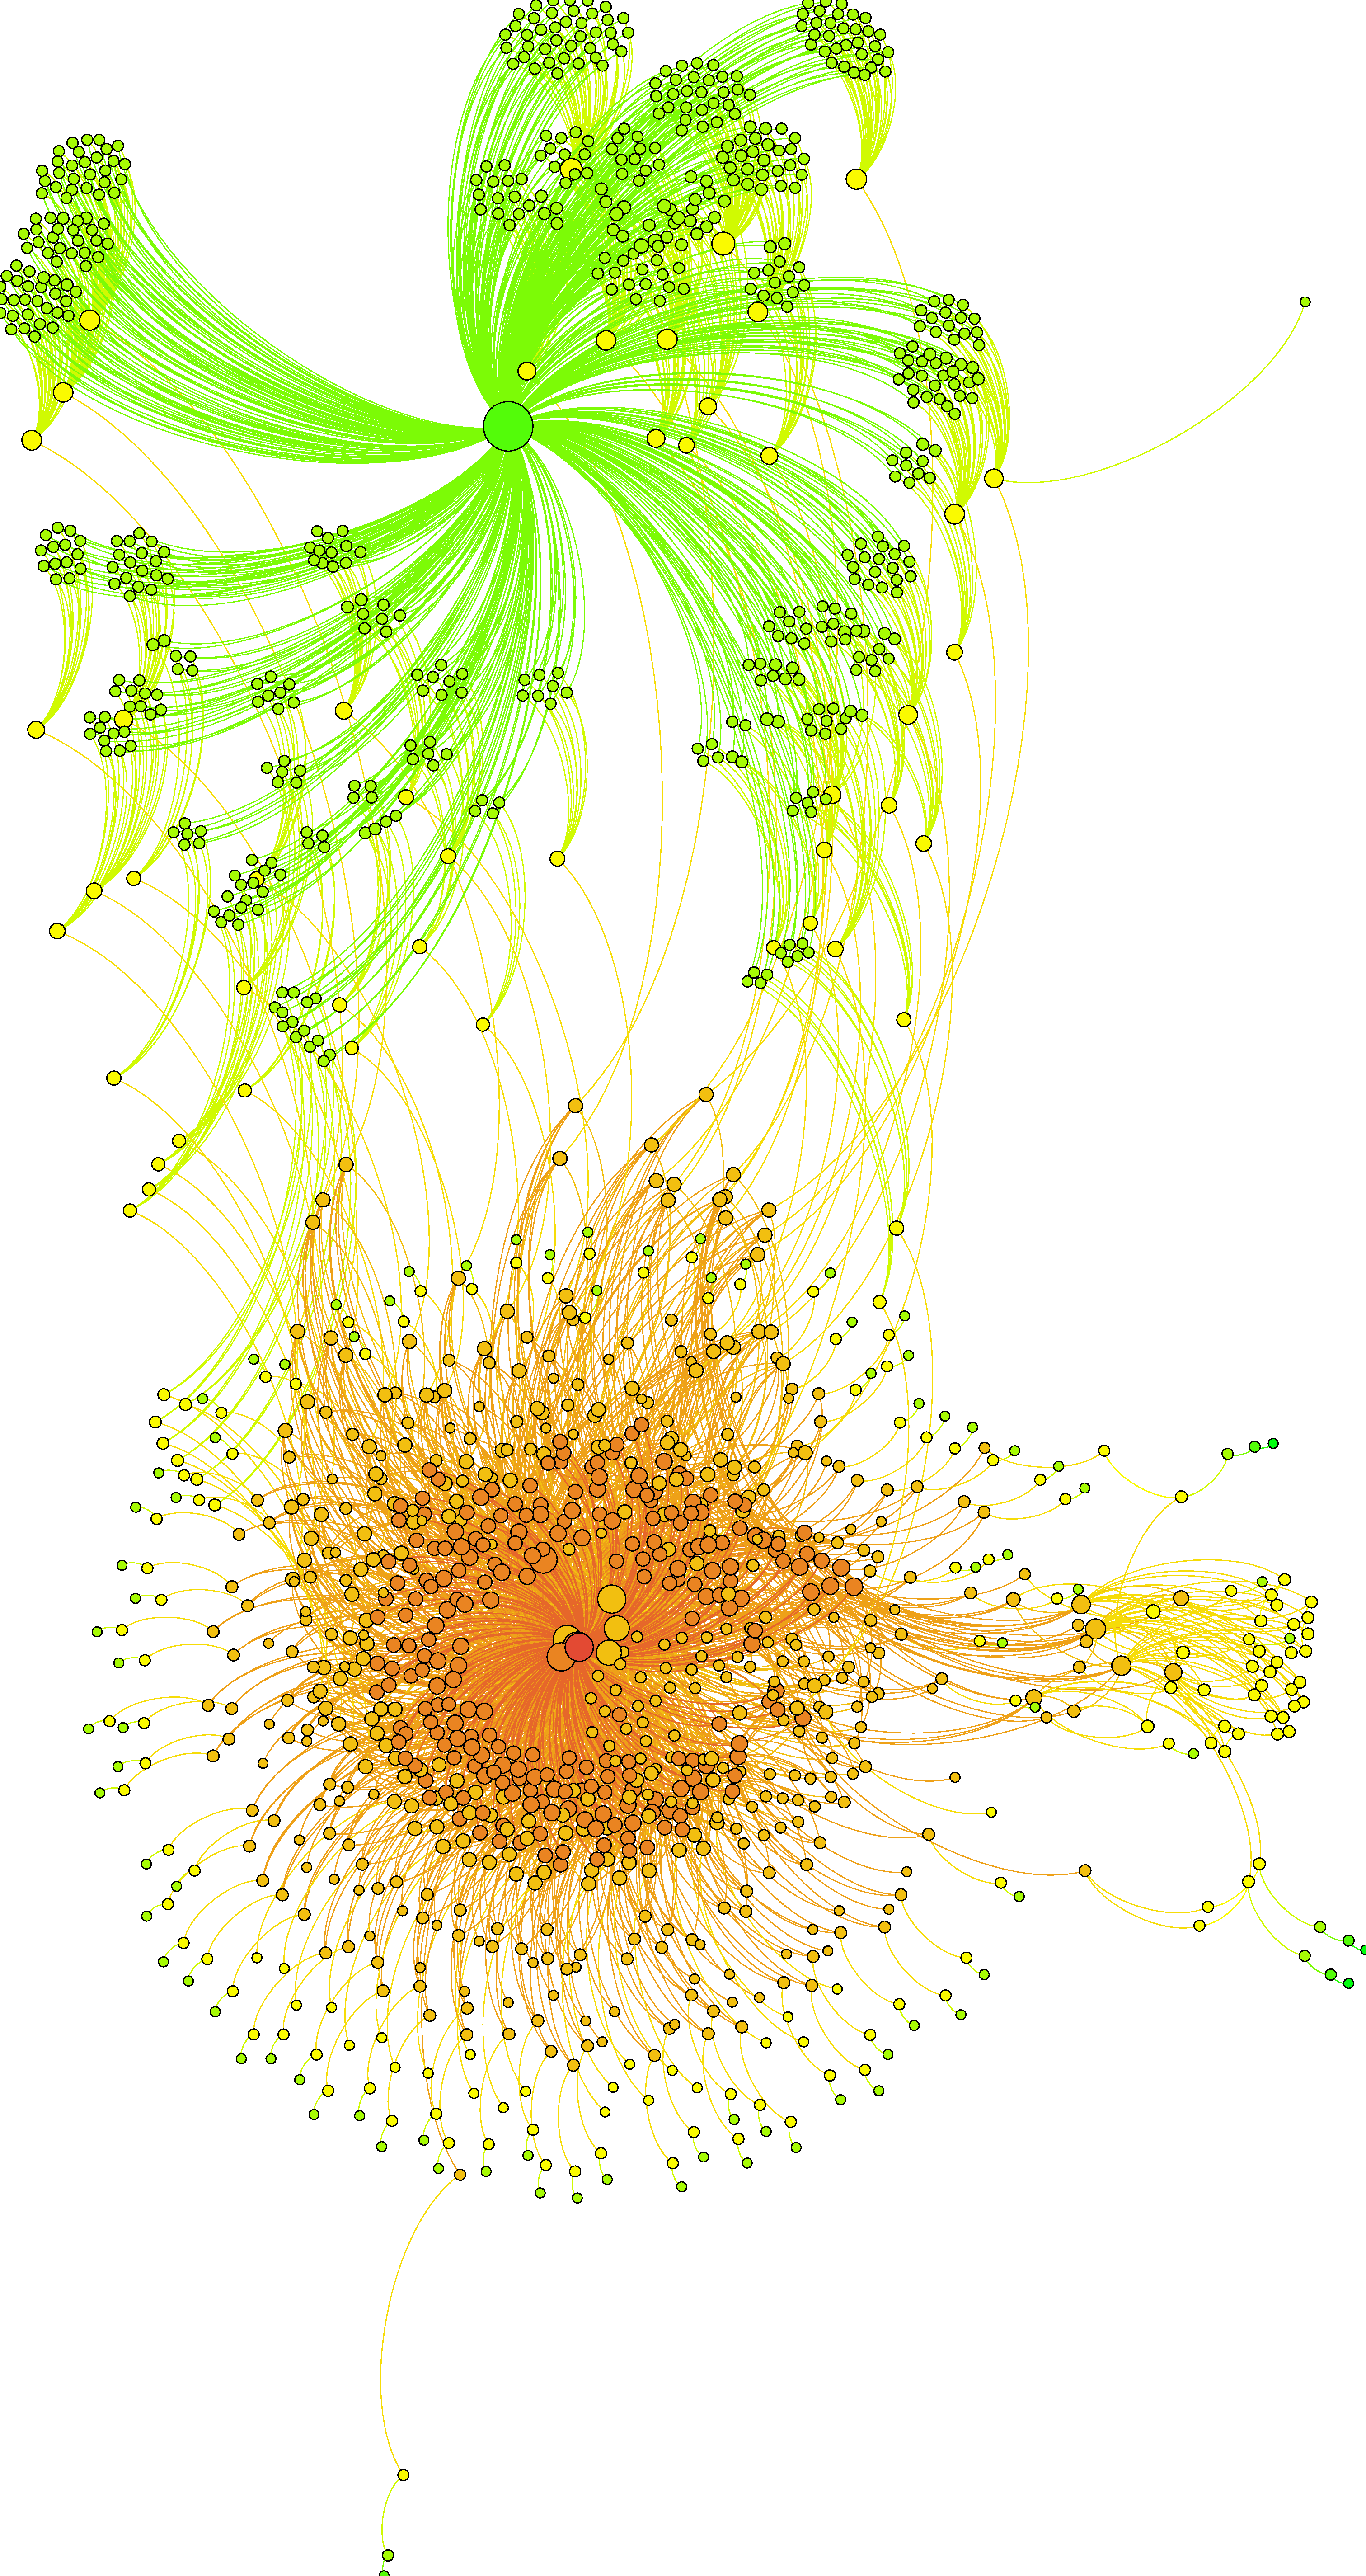
\includegraphics[width=.60\linewidth, angle=90]{book_graph.pdf}
\end{frame}

\begin{frame}{}
    \centering
    \LARGE
    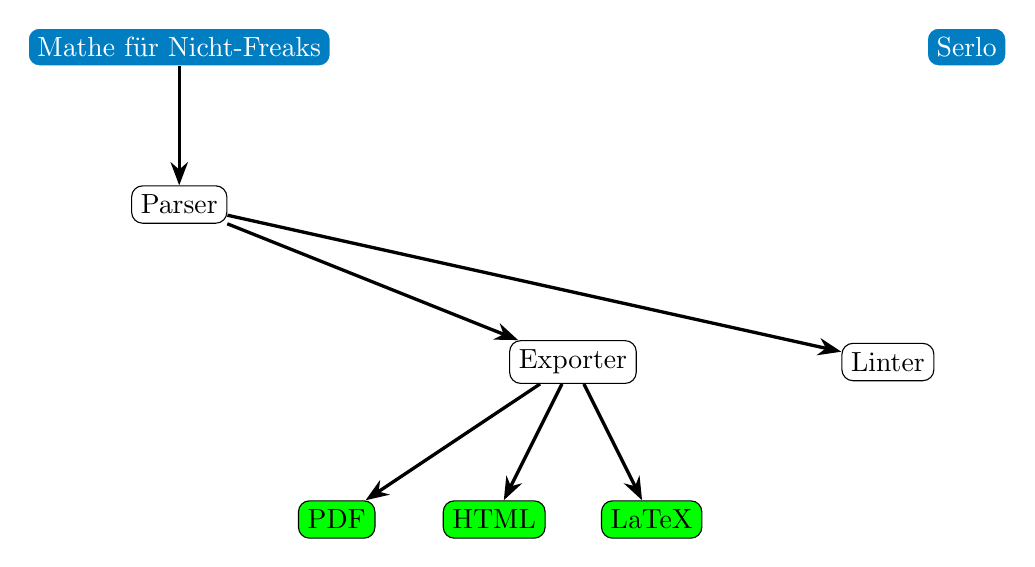
\begin{tikzpicture}[>={Stealth[black]},every edge/.style={draw=black,very thick}]
        \node[draw, rectangle, rounded corners, white, fill=sblau] (W) at (-5, 0) {Mathe für Nicht-Freaks};

        \node[draw, rectangle, rounded corners, white, fill=sblau] (S) at (5, 0) {Serlo};

        \node[draw, rectangle, rounded corners, black] (E) at (0, -4) {Exporter};

        \node[draw, rectangle, rounded corners, black, fill=green] (PDF) at (-3, -6) {PDF};

        \node[draw, rectangle, rounded corners, black, fill=green] (HTML) at (-1, -6) {HTML};

        \node[draw, rectangle, rounded corners, black, fill=green] (LaTeX) at (1, -6) {LaTeX};

        \node[draw, rectangle, rounded corners, black] (P)  at (-5, -2) {Parser};

        \node[draw, rectangle, rounded corners, black] (L) at (4, -4) {Linter};

        \path [->](W) edge (P);
        \path [->](P) edge (E);
        \path [->](P) edge (L);
        
        \path [->](E) edge (PDF);
        \path [->](E) edge (HTML);
        \path [->](E) edge (LaTeX);

    \end{tikzpicture}
\end{frame}

\begin{frame}{}
    \centering
    \LARGE
    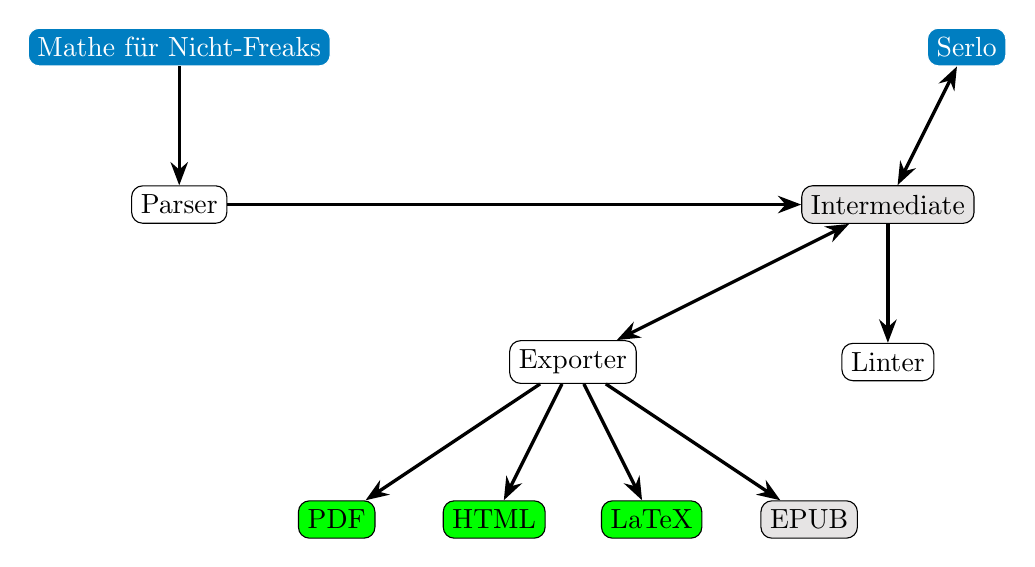
\begin{tikzpicture}[>={Stealth[black]},every edge/.style={draw=black,very thick}]
        \node[draw, rectangle, rounded corners, white, fill=sblau] (W) at (-5, 0) {Mathe für Nicht-Freaks};

        \node[draw, rectangle, rounded corners, white, fill=sblau] (S) at (5, 0) {Serlo};

        \node[draw, rectangle, rounded corners, black] (P)  at (-5, -2) {Parser};

        \node[draw, rectangle, rounded corners, black] (E) at (0, -4) {Exporter};

        \node[draw, rectangle, rounded corners, black, fill=sgrau] (I) at (4, -2) {Intermediate};

        \node[draw, rectangle, rounded corners, black, fill=green] (PDF) at (-3, -6) {PDF};

        \node[draw, rectangle, rounded corners, black, fill=green] (HTML) at (-1, -6) {HTML};

        \node[draw, rectangle, rounded corners, black, fill=green] (LaTeX) at (1, -6) {LaTeX};

        \node[draw, rectangle, rounded corners, black, fill=sgrau] (EPUB) at (3, -6) {EPUB};

        \node[draw, rectangle, rounded corners, black] (L) at (4, -4) {Linter};


        \path [->](W) edge (P);
        
        \path [->](E) edge (PDF);
        \path [->](E) edge (HTML);
        \path [->](E) edge (LaTeX);
        \path [->](E) edge (EPUB);
        \path [->](P) edge (I);
        \path [<->](S) edge (I);
        \path [<->](I) edge (E);
        \path [->](I) edge (L);

    \end{tikzpicture}
\end{frame}

\end{document}
